\documentclass{article}

% chinese fonts
\usepackage{ctex}

% math fonts
\usepackage{amsmath}
\usepackage{amsthm}
\usepackage{amssymb}
\usepackage{bm}

% figures
\usepackage{tikz}
\usepackage{graphicx}
\graphicspath{{./figures/}}

% tables
\usepackage{tabularx}
\usepackage{booktabs}

% codes
\usepackage{listings}

% hyperlinks
\usepackage{hyperref}
\hypersetup{
  breaklinks,
  colorlinks = true,
  citecolor  = blue,
  linkcolor  = red,
  urlcolor   = magenta,
}

% bibliography
\usepackage[sort&compress,numbers]{natbib}

% About:  Macros for Vector, Matrix, Tensor, Math Operator and Misc
% Author: Jingxuan Yang

% vectors
\newcommand{\va}{\bm{a}}       \newcommand{\vah}{\hat{\bm{a}}}        \newcommand{\ah}{\hat{a}}    \newcommand{\vat}{\tilde{\bm{a}}}       \newcommand{\at}{\tilde{a}}
\newcommand{\vb}{\bm{b}}       \newcommand{\vbh}{\hat{\bm{b}}}        \newcommand{\bh}{\hat{b}}    \newcommand{\vbt}{\tilde{\bm{b}}}       \newcommand{\bt}{\tilde{b}}
\newcommand{\vc}{\bm{c}}       \newcommand{\vch}{\hat{\bm{c}}}        \newcommand{\ch}{\hat{c}}    \newcommand{\vct}{\tilde{\bm{c}}}       \newcommand{\ct}{\tilde{c}}
\newcommand{\vd}{\bm{d}}       \newcommand{\vdh}{\hat{\bm{d}}}        \newcommand{\dhat}{\hat{d}}  \newcommand{\vdt}{\tilde{\bm{d}}}       \newcommand{\dt}{\tilde{d}}
\newcommand{\ve}{\bm{e}}       \newcommand{\veh}{\hat{\bm{e}}}        \newcommand{\eh}{\hat{e}}    \newcommand{\vet}{\tilde{\bm{e}}}       \newcommand{\et}{\tilde{e}}
\newcommand{\vf}{\bm{f}}       \newcommand{\vfh}{\hat{\bm{f}}}        \newcommand{\fh}{\hat{f}}    \newcommand{\vft}{\tilde{\bm{f}}}       \newcommand{\ft}{\tilde{f}}
\newcommand{\vg}{\bm{g}}       \newcommand{\vgh}{\hat{\bm{g}}}        \newcommand{\gh}{\hat{g}}    \newcommand{\vgt}{\tilde{\bm{g}}}       \newcommand{\gt}{\tilde{g}}
\newcommand{\vh}{\bm{h}}     \newcommand{\vhh}{\hat{\bm{h}}}        \newcommand{\hh}{\hat{h}}    \newcommand{\vht}{\tilde{\bm{h}}}       \newcommand{\htild}{\tilde{h}}
\newcommand{\vi}{\bm{i}}       \newcommand{\vih}{\hat{\bm{i}}}        \newcommand{\ih}{\hat{i}}    \newcommand{\vit}{\tilde{\bm{i}}}       \newcommand{\itild}{\tilde{i}}
\newcommand{\vj}{\bm{j}}       \newcommand{\vjh}{\hat{\bm{j}}}        \newcommand{\jh}{\hat{j}}    \newcommand{\vjt}{\tilde{\bm{j}}}       \newcommand{\jt}{\tilde{j}}
\newcommand{\vk}{\bm{k}}       \newcommand{\vkh}{\hat{\bm{k}}}        \newcommand{\kh}{\hat{k}}    \newcommand{\vkt}{\tilde{\bm{k}}}       \newcommand{\kt}{\tilde{k}}
\newcommand{\vl}{\bm{l}}       \newcommand{\vlh}{\hat{\bm{l}}}        \newcommand{\lh}{\hat{l}}    \newcommand{\vlt}{\tilde{\bm{l}}}       \newcommand{\lt}{\tilde{l}}
\newcommand{\vm}{\bm{m}}       \newcommand{\vmh}{\hat{\bm{m}}}        \newcommand{\mh}{\hat{m}}    \newcommand{\vmt}{\tilde{\bm{m}}}       \newcommand{\mt}{\tilde{m}}
\newcommand{\vn}{\bm{n}}       \newcommand{\vnh}{\hat{\bm{n}}}        \newcommand{\nh}{\hat{n}}    \newcommand{\vnt}{\tilde{\bm{n}}}       \newcommand{\nt}{\tilde{n}}
\newcommand{\vo}{\bm{o}}       \newcommand{\voh}{\hat{\bm{o}}}        \newcommand{\oh}{\hat{o}}    \newcommand{\vot}{\tilde{\bm{o}}}       \newcommand{\ot}{\tilde{o}}
\newcommand{\vp}{\bm{p}}       \newcommand{\vph}{\hat{\bm{p}}}        \newcommand{\ph}{\hat{p}}    \newcommand{\vpt}{\tilde{\bm{p}}}       \newcommand{\pt}{\tilde{p}}
\newcommand{\vq}{\bm{q}}       \newcommand{\vqh}{\hat{\bm{q}}}        \newcommand{\qh}{\hat{q}}    \newcommand{\vqt}{\tilde{\bm{q}}}       \newcommand{\qt}{\tilde{q}}
\newcommand{\vr}{\bm{r}}       \newcommand{\vrh}{\hat{\bm{r}}}        \newcommand{\rh}{\hat{r}}    \newcommand{\vrt}{\tilde{\bm{r}}}       \newcommand{\rt}{\tilde{r}}
\newcommand{\vs}{\bm{s}}       \newcommand{\vsh}{\hat{\bm{s}}}        \newcommand{\sh}{\hat{s}}    \newcommand{\vst}{\tilde{\bm{s}}}       \newcommand{\st}{\tilde{s}}
\newcommand{\vt}{\bm{t}}       \newcommand{\vth}{\hat{\bm{t}}}        \newcommand{\that}{\hat{t}}  \newcommand{\vtt}{\tilde{\bm{t}}}       \newcommand{\ttil}{\tilde{t}}
\newcommand{\vu}{\bm{u}}       \newcommand{\vuh}{\hat{\bm{u}}}        \newcommand{\uh}{\hat{u}}    \newcommand{\vut}{\tilde{\bm{u}}}       \newcommand{\ut}{\tilde{u}}
\newcommand{\vv}{\bm{v}}       \newcommand{\vvh}{\hat{\bm{v}}}        \newcommand{\vhat}{\hat{v}}    \newcommand{\vvt}{\tilde{\bm{v}}}       \newcommand{\vtild}{\tilde{v}}
\newcommand{\vw}{\bm{w}}       \newcommand{\vwh}{\hat{\bm{w}}}        \newcommand{\wh}{\hat{w}}    \newcommand{\vwt}{\tilde{\bm{w}}}       \newcommand{\wt}{\tilde{w}}
\newcommand{\vx}{\bm{x}}       \newcommand{\vxh}{\hat{\bm{x}}}        \newcommand{\xh}{\hat{x}}    \newcommand{\vxt}{\tilde{\bm{x}}}       \newcommand{\xt}{\tilde{x}}
\newcommand{\vy}{\bm{y}}       \newcommand{\vyh}{\hat{\bm{y}}}        \newcommand{\yh}{\hat{y}}    \newcommand{\vyt}{\tilde{\bm{y}}}       \newcommand{\yt}{\tilde{y}}
\newcommand{\vz}{\bm{z}}       \newcommand{\vzh}{\hat{\bm{z}}}        \newcommand{\zh}{\hat{z}}    \newcommand{\vzt}{\tilde{\bm{z}}}       \newcommand{\zt}{\tilde{z}}

\newcommand{\valpha}{\bm{\alpha}}
\newcommand{\vbeta}{\bm{\beta}}
\newcommand{\vgamma}{\bm{\gamma}}
\newcommand{\vtheta}{\bm{\theta}}
\newcommand{\vlambda}{\bm{\lambda}}
\newcommand{\vmu}{\bm{\mu}}
\newcommand{\vomega}{\bm{\omega}}

\newcommand{\mSigma}{\bm{\Sigma}}

\newcommand{\Fc}{\mathcal{F}}
\newcommand{\Xc}{\mathcal{X}}
\newcommand{\Yc}{\mathcal{Y}}
\newcommand{\Zc}{\mathcal{Z}}
\newcommand{\Gc}{\mathcal{G}}
\newcommand{\Hc}{\mathcal{H}}
\newcommand{\Dc}{\mathcal{D}}
\newcommand{\Cc}{\mathcal{C}}
\newcommand{\Rc}{\mathcal{R}}

% matrices
\newcommand{\ma}{\bm{A}}
\newcommand{\mb}{\bm{B}}
\newcommand{\md}{\bm{D}}
\newcommand{\mH}{\bm{H}}
\newcommand{\mE}{\bm{E}}
\newcommand{\mi}{\bm{I}}
\newcommand{\mk}{\bm{K}}
\newcommand{\ml}{\bm{L}}
\newcommand{\mn}{\bm{N}}
\newcommand{\mP}{\bm{P}}
\newcommand{\mq}{\bm{Q}}
\newcommand{\mr}{\bm{R}}
\newcommand{\mU}{\bm{u}}
\newcommand{\mv}{\bm{v}}
\newcommand{\mw}{\bm{W}}
\newcommand{\mx}{\bm{X}}
\newcommand{\my}{\bm{Y}}
\newcommand{\mz}{\bm{Z}}

% tensors
\newcommand{\tp}{\mathsf{P}}
\newcommand{\tu}{\mathsf{U}}
\newcommand{\tx}{\mathsf{X}}
\newcommand{\ty}{\mathsf{Y}}
\newcommand{\tz}{\mathsf{Z}}
\newcommand{\tw}{\mathsf{W}}
\newcommand{\tf}{\mathsf{F}}
\newcommand{\ta}{\mathsf{A}}
\renewcommand{\th}{\mathsf{H}}

% norms
\newcommand{\mynorm}[2]{\| {#1} \|_{#2}}
\newcommand{\norm}[2]{\mynorm{#1}{#2}}
\newcommand{\bignorm}[2]{\left\| {#1} \right\|_{#2}}
\newcommand{\norml}[1]{\mynorm{#1}{1}}
\newcommand{\bignorml}[1]{\bignorm{#1}{1}}
\newcommand{\infnorm}[1]{\mynorm{#1}{\infty}}
\newcommand{\biginfnorm}[1]{\bignorm{#1}{\infty}}
\newcommand{\oneinf}{\ell_{1,\infty}}
\newcommand{\onetwo}{\ell_{1,2}}
\newcommand{\oneinfnorm}[1]{\mynorm{#1}{1,\infty}}
\newcommand{\bigoneinf}[1]{\bignorm{#1}{1,\infty}}
\newcommand{\onetwonorm}[1]{\mynorm{#1}{1,2}}
\newcommand{\bigonetwo}[1]{\bignorm{#1}{1,2}}
\newcommand{\enorm}[1]{\mynorm{#1}{2}}
\newcommand{\bigenorm}[1]{\bignorm{#1}{2}}
\newcommand{\znorm}[1]{\mynorm{#1}{0}}
\newcommand{\bigznorm}[1]{\bignorm{#1}{0}}
\newcommand{\frob}[1]{\|{#1}\|_{\text{F}}}
\newcommand{\bigfrob}[1]{\bignorm{#1}{\text{F}}}
\newcommand{\grpnorm}[2]{\norm{#1}{\text{Gr}(#2)}}

% math operators
\DeclareMathOperator*{\argmin}{argmin}
\DeclareMathOperator*{\argmax}{argmax}
\DeclareMathOperator{\divg}{div}
\DeclareMathOperator{\dom}{dom}
\DeclareMathOperator{\interior}{int}
\DeclareMathOperator{\ri}{ri}
\DeclareMathOperator{\sgn}{sgn}
\DeclareMathOperator{\trace}{Tr}
\DeclareMathOperator{\diag}{diag}
\DeclareMathOperator{\rank}{rank}
\DeclareMathOperator{\range}{range}
\DeclareMathOperator{\vect}{vec}
\DeclareMathOperator{\prox}{prox}
\DeclareMathOperator{\intr}{int}
\DeclareMathOperator{\relint}{ri}

% misc
\newcommand{\gs}{\geqslant}
\newcommand{\ls}{\leqslant}
\newcommand{\set}[1]{\left\{ {#1}\right\}}

\newcommand{\defeq}{\ \stackrel{\text{def}}{=}\ }
\newcommand{\ip}[2]{\left\langle#1, #2\right\rangle}
\newcommand{\reals}{\mathbb{R}}
\newcommand{\complex}{\mathbb{C}}
\newcommand{\half}{\frac{1}{2}}

\newtheorem{theorem}{Theorem}
\newtheorem{lemma}[theorem]{Lemma}
\newtheorem{proposition}[theorem]{Proposition}
\newtheorem{remark}[theorem]{Remark}
\newtheorem{corollary}[theorem]{Corollary}
\newtheorem{definition}[theorem]{Definition}


\setlength{\oddsidemargin}{-0.25 in}
\setlength{\evensidemargin}{-0.25 in} 
\setlength{\topmargin}{-0.25in} 
\setlength{\textwidth}{7 in} 
\setlength{\textheight}{8.5 in}
\setlength{\headsep}{0.25 in} 
\setlength{\parindent}{0 in}
\setlength{\parskip}{0.1 in}

\newcommand{\homework}[5]{
  \pagestyle{myheadings} 
  \thispagestyle{plain}
  \newpage
  \setcounter{page}{1} 
  \setcounter{section}{#5} 
  \noindent
  \begin{center}
    \framebox{ 
      \vbox{
        \vspace{2mm} 
        \hbox to 6.28in { {\bf
        THU-70250043-0,~Pattern~Recognition~(Spring 2021) \hfill Homework: 2} }
        \vspace{6mm} 
        \hbox to 6.28in { {\Large \hfill #1 \hfill} }
        \vspace{6mm} 
        \hbox to 6.28in { {\it Lecturer: #2 \hfill} }
        \vspace{2mm} 
        \hbox to 6.28in { {\it \hspace{14mm} #3 \hfill} }
        \vspace{2mm} 
        \hbox to 6.28in { {\it Student: #4 \hfill} }
        \vspace{2mm} 
      } 
    }
  \end{center}
  \markboth{#1}{#1} 
  \vspace*{4mm} 
}

\begin{document}

\homework{Density Estimation}{Changshui Zhang
\hspace{5mm} {\tt zcs@mail.tsinghua.edu.cn}}{Hong Zhao \hspace{16mm} {\tt vzhao@tsinghua.edu.cn}}{Jingxuan Yang \hspace{10mm} {\tt yangjx20@mails.tsinghua.edu.cn}}{8}

\section*{Maximum likelihood and Bayesian parameter estimation}

1. Let $x$ have an exponential density
\begin{equation}
  p(x|\theta)=
  \left\{
    \begin{array}{ll}
      \theta e^{-\theta x}, & x \gs 0 \\
      0,                    & \text {otherwise.}
    \end{array}
  \right.
\end{equation}

1.1 Plot $p(x|\theta)$ versus $x$ for $\theta = 1$. Plot $p(x|\theta)$ versus $\theta$, ($0 \ls \theta \ls 5$) for $x = 2$.

解: 分别如图 \ref{fig:epdf1} 和图 \ref{fig:epdf2} 所示.

\begin{figure}[htbp]
  \centering
  \begin{minipage}[t]{0.48\textwidth}
  \centering
  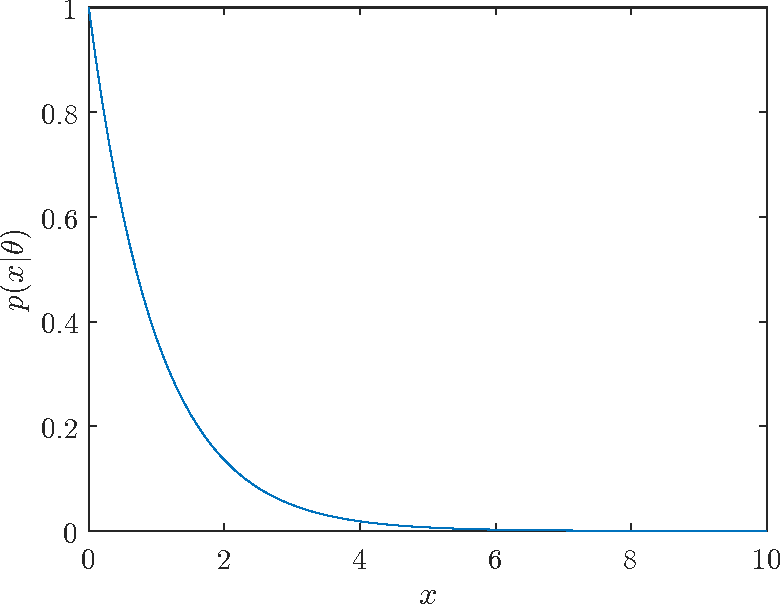
\includegraphics[width=8cm]{epdf-1.pdf}
  \caption{$p(x|\theta)$ 关于 $x$ 曲线}
  \label{fig:epdf1}
  \end{minipage}
  \begin{minipage}[t]{0.48\textwidth}
  \centering
  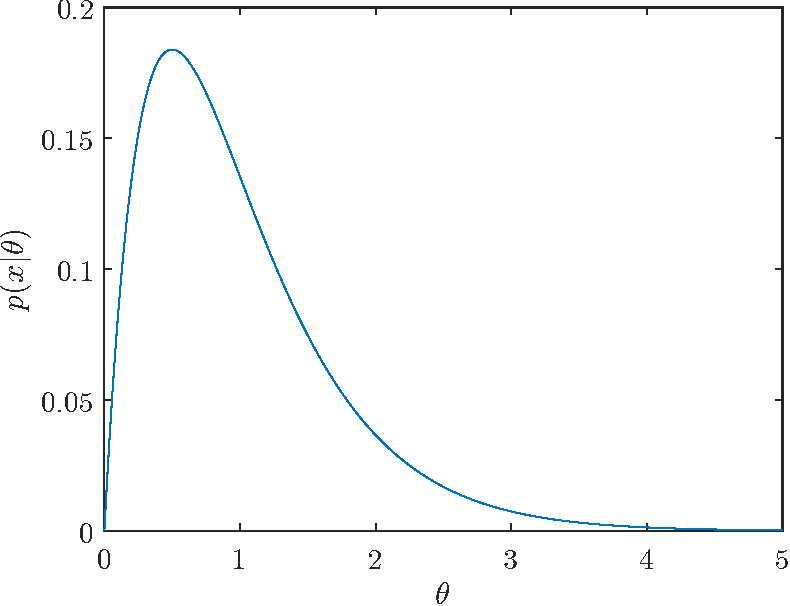
\includegraphics[width=8cm]{epdf-2.pdf}
  \caption{$p(x|\theta)$ 关于 $\theta$ 曲线}
  \label{fig:epdf2}
  \end{minipage}
\end{figure}

1.2 Suppose that $n$ samples ${x_1, \cdots, x_n}$ are drawn independently according to $p(x|\theta)$.
Calculate the maximum likelihood estimate for $\theta$.

解: $\theta$ 的最大似然估计应该是下面方程的解
\begin{equation}
  \nabla_\theta H(\theta)=\sum_{k=1}^n\nabla_\theta\ln p(x_k|\theta)=0
\end{equation}

由指数分布可知
\begin{equation}
  \ln p(x_k|\theta)=\ln\theta-\theta x_k,\quad\forall~k=1,2,\cdots,n
\end{equation}

其梯度为
\begin{equation}
  \nabla_\theta\ln p(x_k|\theta)=\frac{1}{\theta}-x_k,\quad\forall~k=1,2,\cdots,n
\end{equation}

因此 $\theta$ 的最大似然估计满足
\begin{equation}
  \sum_{k=1}^n\left(\frac{1}{\hat{\theta}}-x_k\right)=0
\end{equation}

故 $\theta$ 的最大似然估计为
\begin{equation}
  \hat{\theta}=\frac{1}{\displaystyle\frac{1}{n}\sum_{k=1}^nx_k}
\end{equation}

2. The purpose of this problem is to derive the Bayesian classifier for the $d$-dimensional multivariate Bernoulli case. Let $x$ be a $d$-dimensional binary (0 or 1) vector with a multivariate Bernoulli distribution.
\begin{equation}
  p(\bm{x}|\bm{\theta})
  =\prod_{i=1}^{d} \theta_{i}^{x_{i}}\left(1-\theta_{i}\right)^{1-x_{i}},
\end{equation}
where $\bm{\theta}=\left(\theta_{1}, \cdots, \theta_{d}\right)^{T}$ is an unknown parameter vector, $\theta_i$ being the probablility that $x_i=1$. Let $\mathcal{D}$ be a set of $n$ samples $\bm{x}_1, \cdots, \bm{x}_n$ independently drawn according to $p(\bm{x}|\bm{\theta})$. Denote $P\left(\bm{x}_{1}, \cdots, \bm{x}_{n}|\bm{\theta}\right)$ as $P(\mathcal{D}|\bm{\theta})$.

2.1 Calculate the maximum likelihood estimate for $\bm{\theta}$.

解: $\bm{\theta}$ 的最大似然估计应该是下面方程的解
\begin{equation}
  \nabla_{\bm{\theta}} H(\bm{\theta})=\sum_{k=1}^n\nabla_{\bm{\theta}}\ln p(\bm{x}_k|\bm{\theta})=\bm{0}
\end{equation}

由分布函数可知
\begin{equation}
  \ln p(\bm{x}_k|\bm{\theta})=\sum_{i=1}^d\big[x_{k,i}\ln\theta_i+(1-x_{k,i})\ln(1-\theta_i)\big],\quad\forall~k=1,2,\cdots,n
\end{equation}

其对 $\theta_i$ 的梯度为
\begin{equation}
  \nabla_{\theta_i}\ln p(\bm{x}_k|\bm{\theta})=\frac{x_{k,i}}{\theta_i}-\frac{1-x_{k,i}}{1-\theta_i},\quad\forall~k=1,2,\cdots,n,~\forall~i=1,2,\cdots,d
\end{equation}

因此
\begin{equation}
  \sum_{k=1}^n\left(\frac{x_{k,i}}{\theta_i}-\frac{1-x_{k,i}}{1-\theta_i}\right)=0,\quad\forall~i=1,2,\cdots,d
\end{equation}

故 $\theta_i$ 的最大似然估计满足
\begin{equation}
  (1-\hat{\theta}_i)\sum_{k=1}^nx_{k,i}=\hat{\theta}_i\sum_{k=1}^n(1-x_{k,i})=\hat{\theta}_i\left(n-\sum_{k=1}^nx_{k,i}\right),\quad\forall~i=1,2,\cdots,d
\end{equation}

化简得
\begin{equation}
  \hat{\theta}_i=\frac{1}{n}\sum_{k=1}^nx_{k,i},\quad\forall~i=1,2,\cdots,d
\end{equation}

写成向量形式为
\begin{equation}
  \hat{\bm{\theta}}=\frac{1}{n}\sum_{k=1}^n\vx_k
\end{equation}

2.2 Assuming a uniform a priori distribution for $\bm{\theta}$, $0 \ls {\theta}_i \ls 1$, and using the identity
\begin{equation}
  \int_{0}^{1} \theta^{m}(1-\theta)^{n} \mathrm{d}\theta=\frac{m ! n !}{(m+n+1) !},
\end{equation}
calculate the probablility $p(\bm{\theta}|\mathcal{D})$.

解: 令 $\bm{s}$ 表示 $n$ 个样本的和, 即
\begin{equation}
  \bm{s}=\sum_{k=1}^n\vx_k
\end{equation}

则 $P(\mathcal{D}|\bm{\theta})$ 可以计算为
\begin{equation}
  \begin{aligned}
    P(\mathcal{D}|\bm{\theta})
    &=\prod_{k=1}^np(\vx_k|\vtheta)\\
    &=\prod_{k=1}^n\prod_{i=1}^d \theta_{i}^{x_{k,i}}\left(1-\theta_{i}\right)^{1-x_{k,i}}\\
    &=\prod_{i=1}^d\theta_{i}^{s_{i}}\left(1-\theta_{i}\right)^{n-s_{i}}\\
  \end{aligned}
\end{equation}

所以 $p(\mathcal{D})$ 为
\begin{equation}
  \begin{aligned}
    p(\mathcal{D})
    &=\int_{[0,1]^d} P(\mathcal{D}|\bm{\theta})p(\vtheta)\mathrm{d}\vtheta\\
    &=\int_0^1\int_0^1\cdots\int_0^1 \prod_{i=1}^d\theta_{i}^{s_{i}}\left(1-\theta_{i}\right)^{n-s_{i}}\mathrm{d}\theta_1\mathrm{d}\theta_2\cdots\mathrm{d}\theta_d\\
    &=\prod_{i=1}^d\frac{s_i!(n-s_i)!}{(n+1)!}\\
  \end{aligned}
\end{equation}

所以由 Bayes 公式可得概率 $p(\bm{\theta}|\mathcal{D})$ 为
\begin{equation}
  \begin{aligned}
    p(\bm{\theta}|\mathcal{D})
    &=\frac{p(\vtheta,\mathcal{D})}{p(\mathcal{D})}\\
    &=\frac{P(\mathcal{D}|\bm{\theta})p(\vtheta)}{p(\mathcal{D})}\\
    &=\prod_{i=1}^d\frac{(n+1)!}{s_i!(n-s_i)!}\theta_{i}^{s_{i}}\left(1-\theta_{i}\right)^{n-s_{i}}\\
  \end{aligned}
\end{equation}

2.3 Integrate the product $p(\bm{x}|\bm{\theta}) p(\bm{\theta}|\mathcal{D})$ over $\bm{\theta}$ to obtain the desired probability $p(\bm{x}|\mathcal{D})$.

解: 注意到 $x_i\in\{0,1\}$ 则有
\begin{equation}
  \begin{aligned}
    p(\bm{x}|\mathcal{D})
    &=\int_{[0,1]^d} p(\bm{x}|\bm{\theta}) p(\bm{\theta}|\mathcal{D})\mathrm{d}\vtheta\\
    &=\int_{[0,1]^d} \prod_{i=1}^{d} \theta_{i}^{x_{i}}(1-\theta_{i})^{1-x_{i}} \prod_{i=1}^d\frac{(n+1)!}{s_i!(n-s_i)!}\theta_{i}^{s_{i}}(1-\theta_{i})^{n-s_{i}}\mathrm{d}\vtheta\\
    &=\int_0^1\int_0^1\cdots\int_0^1 \prod_{i=1}^{d}\frac{(n+1)!}{s_i!(n-s_i)!}\theta_{i}^{s_{i}+x_{i}}(1-\theta_{i})^{n+1-s_{i}-x_i}\mathrm{d}\theta_1\mathrm{d}\theta_2\cdots\mathrm{d}\theta_d\\
    &=\prod_{i=1}^{d}\frac{(n+1)!}{s_i!(n-s_i)!}\frac{(s_i+x_i)!(n+1-s_i-x_i)!}{(n+2)!}\\
    &=\prod_{i=1}^{d}\frac{1}{n+2}\frac{(s_i+x_i)!}{s_i!}\frac{(n+1-s_i-x_i)!}{(n-s_i)!}\\
    &=\prod_{i=1}^{d}\frac{1}{n+2}(s_i+x_i)^{x_i}(n+1-s_i-x_i)^{1-x_i},\quad x_i\in\{0,1\}\\
    &=\prod_{i=1}^{d}\frac{1}{n+2}(s_i+1)^{x_i}(n+1-s_i)^{1-x_i},\quad x_i\in\{0,1\}\\
    &=\prod_{i=1}^{d}\left(\frac{s_i+1}{n+2}\right)^{x_i}\left(1-\frac{s_i+1}{n+2}\right)^{1-x_i}\\
  \end{aligned}
\end{equation}

2.4 If we think of obtaining $p(\bm{x}|\mathcal{D})$ by substituting an estimate $\hat{\bm{\theta}}$ for $\bm{\theta}$ in $p(\bm{x}|\bm{\theta})$,
what is the effective Bayesian estimate for $\bm{\theta}$?

解: 已知
\begin{equation}
  p(\bm{x}|\bm{\theta})
  =\prod_{i=1}^{d} \theta_{i}^{x_{i}}\left(1-\theta_{i}\right)^{1-x_{i}}
\end{equation}

且由上题有

\begin{equation}
  p(\bm{x}|\mathcal{D})=\prod_{i=1}^{d}\left(\frac{s_i+1}{n+2}\right)^{x_i}\left(1-\frac{s_i+1}{n+2}\right)^{1-x_i}
\end{equation}

根据以上两式, 不难看出参数 $\vtheta$ 的 Bayes 估计为
\begin{equation}
  \hat{\vtheta}_B=\frac{\vs+1}{n+2}=\frac{1}{n+2}\left(\sum_{k=1}^nx_k+1\right)
\end{equation}

2.5 When do maximum likelihood estimation and Bayesian estimation methods differ. (Describe in your own words, not limited to the above examples.)

解: 当训练样本数无穷多的时候, 最大似然估计与 Bayes 估计的结果是一样的, 否则, 他们的结果是不同的.

3. Prove the invariance property of maximum likelihood estimators, i.e., that if $\hat{\theta}$ is the maximum likelihood estimate of $\theta$, then for any differentiable function $\tau(\cdot)$, the maximum likelihood estimate of $\tau(\theta)$ is $\tau(\hat{\theta})$.

证明: 对 $\tau(\theta)$, 文献 \cite{b1} 基于似然函数 $L(\theta|x)$ 定义导出似然函数 (induced likelihood function) $L^*$ 为
\begin{equation}
  L^*(\eta|x)=\sup_{\{\theta:\tau(\theta)=\eta\}}L(\theta|x)
\end{equation}

令 $\hat{\eta}$ 表示使得导出似然函数取到最大值的变量, 即
\begin{equation}
  \hat{\eta}=\argmax_\eta L^*(\eta|x)
\end{equation}

所以由导出似然函数的定义和最大似然估计的定义可得
\begin{equation}
  \begin{aligned}
    L^*(\hat{\eta}|x)
    &=\sup_\eta\sup_{\{\theta:\tau(\theta)=\eta\}}L(\theta|x)\\
    &=\sup_\theta L(\theta|x)\\
    &=L(\hat{\theta}|x)\\
  \end{aligned}
\end{equation}

又由 $\hat{\theta}$ 是 $\theta$ 的最大似然估计可得
\begin{equation}
  \begin{aligned}
    L(\hat{\theta}|x)
    &=\sup_{\{\theta:\tau(\theta)=\tau(\hat{\theta})\}}L(\theta|x)\\
    &=L^*[\tau(\hat{\theta})|x]
  \end{aligned}
\end{equation}

则
\begin{equation}
  L^*(\hat{\eta}|x)=L^*[\tau(\hat{\theta})|x]
\end{equation}

因此 $\tau(\hat{\theta})$ 是 $\tau(\theta)$ 的最大似然估计.

\section*{Nonparametric density estimation}

4. Consider a normal $p(x)\sim N(\mu,\sigma^2)$ and Parzen-window function ${\varphi(x) \sim N(0,1)}$. Show that the Parzen-window estimate
\begin{equation}
  p_{n}(x)=\frac{1}{nh_n} \sum_{i=1}^{n} \varphi\left(\frac{x-x_{i}}{h_{n}}\right)
\end{equation}
has the following properties for small $h_{n}$:

4.1 $\bar{p}_n(x)\sim N(\mu,\sigma^2+h_n^2)$.

解: 令
\begin{equation}
  \theta^2\triangleq\frac{1}{\dfrac{1}{h_n^2}+\dfrac{1}{\sigma^2}}=\frac{h_n^2\sigma^2}{h_n^2+\sigma^2}
\end{equation}
且
\begin{equation}
  \alpha\triangleq\theta^2\left(\frac{x}{h_n^2}+\frac{\mu}{\sigma^2}\right)
\end{equation}

则期望值为
\begin{equation}
  \begin{aligned}
    \bar{p}_{n}(x)
    &=\mathbb{E}[p_n(x)]\\
    &=\frac{1}{nh_n}\sum_{i=1}^n\mathbb{E}\left[\varphi\left(\frac{x-x_{i}}{h_{n}}\right)\right]\\
    &=\frac{1}{h_n}\int_{-\infty}^\infty\varphi\left(\frac{x-v}{h_{n}}\right)p(v)\mathrm{d}v\\
    &=\frac{1}{h_n}\int_{-\infty}^\infty\frac{1}{\sqrt{2\pi}}\exp\left[-\frac{1}{2}\left(\frac{x-v}{h_n}\right)^2\right]\frac{1}{\sqrt{2\pi}\sigma}\exp\left[-\frac{1}{2}\left(\frac{v-\mu}{\sigma}\right)^2\right]\mathrm{d}v\\
    &=\frac{1}{2\pi h_n\sigma}\exp\left[-\frac{1}{2}\left(\frac{x^2}{h_n^2}+\frac{\mu^2}{\sigma^2}\right)\right]\int_{-\infty}^\infty\exp\left\{-\frac{1}{2}\left[v^2\left(\frac{1}{h_n^2}+\frac{1}{\sigma^2}\right)-2v\left(\frac{x}{h_n^2}+\frac{\mu}{\sigma^2}\right)\right]\right\}\mathrm{d}v\\
    &=\frac{1}{2\pi h_n\sigma}\exp\left[-\frac{1}{2}\left(\frac{x^2}{h_n^2}+\frac{\mu^2}{\sigma^2}\right)+\frac{1}{2}\frac{\alpha^2}{\theta^2}\right]\int_{-\infty}^\infty\exp\left[-\frac{1}{2}\left(\frac{v-\alpha}{\theta}\right)^2\right]\mathrm{d}v\\
    &=\frac{\sqrt{2\pi}\theta}{2\pi h_n\sigma}\exp\left[-\frac{1}{2}\left(\frac{x^2}{h_n^2}+\frac{\mu^2}{\sigma^2}-\frac{\alpha^2}{\theta^2}\right)\right]\\
    &=\frac{1}{\sqrt{2\pi}h_n\sigma}\frac{h_n\sigma}{\sqrt{h_n^2+\sigma^2}}\exp\left[-\frac{1}{2}\left(\frac{x^2\sigma^2+h_n^2\mu^2}{h_n^2\sigma^2}-\frac{h_n^2\sigma^2}{h_n^2+\sigma^2}\frac{(x\sigma^2+h_n^2\mu)^2}{(h_n^2\sigma^2)^2}\right)\right]\\
    &=\frac{1}{\sqrt{2\pi}\sqrt{h_n^2+\sigma^2}}\exp\left[-\frac{1}{2}\frac{(x^2\sigma^2+h_n^2\mu^2)(h_n^2+\sigma^2)-(x\sigma^2+h_n^2\mu)^2}{h_n^2\sigma^2(h_n^2+\sigma^2)}\right]\\
    &=\frac{1}{\sqrt{2\pi}\sqrt{h_n^2+\sigma^2}}\exp\left[-\frac{1}{2}\frac{x^2\sigma^2h_n^2+\mu^2h_n^2\sigma^2-2x\mu h_n^2\sigma^2}{h_n^2\sigma^2(h_n^2+\sigma^2)}\right]\\
    &=\frac{1}{\sqrt{2\pi}\sqrt{h_n^2+\sigma^2}}\exp\left[-\frac{1}{2}\left(\frac{x-\mu}{\sqrt{h_n^2+\sigma^2}}\right)^2\right]\\
  \end{aligned}
\end{equation}

因此
\begin{equation}
  \bar{p}_n(x)\sim N(\mu,\sigma^2+h_n^2)
\end{equation}

4.2 $\text{Var}[p_n(x)]\simeq\dfrac{1}{2nh_n\sqrt{\pi}}p(x)$.

解: 由 4.1 可知, 当 $h_n$ 充分小时, 有
\begin{equation}
  \bar{p}_n(x)\sim N(\mu,\sigma^2)
\end{equation}

即有
\begin{equation}
  \frac{1}{h_n}\mathbb{E}\left[\varphi\left(\frac{x-v}{h_{n}}\right)\right]\simeq p(x)
\end{equation}

则当 $h_n$ 充分小时, 利用上述结论以及 $x_1,x_2,\cdots,x_n$ 的独立性可得方差为
\begin{equation}
  \begin{aligned}
    \text{Var}[p_n(x)]
    &=\text{Var}\left[\frac{1}{nh_n}\sum_{i=1}^{n} \varphi\left(\frac{x-x_{i}}{h_{n}}\right)\right]\\
    &=\frac{1}{n^2h_n^2}\sum_{i=1}^{n}\text{Var} \left[\varphi\left(\frac{x-x_{i}}{h_{n}}\right)\right]\\
    &=\frac{1}{nh_n^2}\text{Var} \left[\varphi\left(\frac{x-v}{h_{n}}\right)\right]\\
    &=\frac{1}{nh_n^2}\left\{\mathbb{E}\left[\varphi^2\left(\frac{x-v}{h_{n}}\right)\right]-\mathbb{E}^2\left[\varphi\left(\frac{x-v}{h_{n}}\right)\right]\right\}\\
    &=\frac{1}{nh_n^2}\left\{\frac{1}{\sqrt{2\pi}}\mathbb{E}\left[\varphi\left(\frac{x-v}{h_{n}/\sqrt{2}}\right)\right]-\mathbb{E}^2\left[\varphi\left(\frac{x-v}{h_{n}}\right)\right]\right\}\\
    &=\frac{1}{2nh_n\sqrt{\pi}}\frac{1}{h_n/\sqrt{2}}\mathbb{E}\left[\varphi\left(\frac{x-v}{h_{n}/\sqrt{2}}\right)\right]-\frac{1}{n}\left\{\frac{1}{h_n}\mathbb{E}\left[\varphi\left(\frac{x-v}{h_{n}}\right)\right]\right\}^2\\
    &\simeq\frac{p(x)}{2nh_n\sqrt{\pi}}\Big[1-2\sqrt{\pi}h_np(x)\Big]\\
    &\simeq\frac{p(x)}{2nh_n\sqrt{\pi}}
  \end{aligned}
\end{equation}

4.3 $\displaystyle p(x)-\bar{p}_{n}(x) \simeq \frac{1}{2}\left(\frac{h_{n}}{\sigma}\right)^{2}\left[1-\left(\frac{x-\mu}{\sigma}\right)^{2}\right] p(x)$.

解: 偏差为
\begin{equation}
  \begin{aligned}
    p(x)-\bar{p}_n(x)
    &=p(x)\left[1-\frac{\bar{p}_n(x)}{p(x)}\right]\\
    &=p(x)\left\{1-\frac{\sigma}{\sqrt{\sigma^2+h_n^2}}\exp\left[-\frac{1}{2}\frac{(x-\mu)^2}{\sigma^2+h_n^2}+\frac{1}{2}\frac{(x-\mu)^2}{\sigma^2}\right]\right\}\\
    &=p(x)\left\{1-\frac{1}{\sqrt{1+(h_n/\sigma)^2}}\exp\left[\frac{1}{2}\frac{h_n^2}{\sigma^2}\frac{(x-\mu)^2}{\sigma^2+h_n^2}\right]\right\}\\
  \end{aligned}
\end{equation}

当 $h_n$ 充分小时, 有
\begin{equation}
  \frac{1}{\sqrt{1+(h_n/\sigma)^2}}\simeq 1-\frac{1}{2}\frac{h_n^2}{\sigma^2}
\end{equation}

和
\begin{equation}
  \exp\left[\frac{1}{2}\frac{h_n^2}{\sigma^2}\frac{(x-\mu)^2}{\sigma^2+h_n^2}\right]\simeq 1+\frac{1}{2}\frac{h_n^2}{\sigma^2}\frac{(x-\mu)^2}{\sigma^2+h_n^2}
\end{equation}

所以
\begin{equation}
  \begin{aligned}
    p(x)-\bar{p}_n(x)
    &\simeq p(x)\left[1-\left(1-\frac{1}{2}\frac{h_n^2}{\sigma^2}\right)\left(1+\frac{1}{2}\frac{h_n^2}{\sigma^2}\frac{(x-\mu)^2}{\sigma^2+h_n^2}\right)\right]\\
    &\simeq p(x)\left[1-1+\frac{1}{2}\frac{h_n^2}{\sigma^2}-\frac{1}{2}\frac{h_n^2}{\sigma^2}\frac{(x-\mu)^2}{\sigma^2+h_n^2}\right]\\
    &=\frac{1}{2}\frac{h_n^2}{\sigma^2}p(x)\left[1-\frac{(x-\mu)^2}{\sigma^2+h_n^2}\right]\\
    &\simeq \frac{1}{2}\left(\frac{h_{n}}{\sigma}\right)^{2}\left[1-\left(\frac{x-\mu}{\sigma}\right)^{2}\right] p(x)\\
  \end{aligned}
\end{equation}

5. Consider classifiers based on samples from the distributions
\begin{equation}
  p\left(x|\omega_{1}\right)=
  \left\{
    \begin{array}{ll}
      3 / 2, & \text { for } 0 \ls x \ls 2 / 3 \\
      0,     & \text { otherwise }
    \end{array}
  \right.
\end{equation}
and
\begin{equation}
  p\left(x|\omega_{2}\right)=
  \left\{
    \begin{array}{ll}
      3 / 2, & \text { for } 1 / 3 \ls x \ls 1 \\
      0,     & \text { otherwise. }
    \end{array}
  \right.
\end{equation}

5.1  What is the Bayes decision rule and the Bayes classification error?

解: 假定 $P(\omega_1)=P(\omega_2)$, 则边界点
\begin{equation}
  t\in\left[\frac{1}{3},~\frac{2}{3}\right]
\end{equation}

取定 $t$, 则 Bayes 决策为
\begin{equation}
  \begin{aligned}
    x\in(0,t)&\to x\in\omega_1\\
    x\in(t,1)&\to x\in\omega_2\\
  \end{aligned}
\end{equation}

Bayes 决策错误率为
\begin{equation}
  \begin{aligned}
    P_B(e)
    &=P(\omega_1)\int_{t}^1p(x|\omega_1)\mathrm{d}x+P(\omega_2)\int_{0}^tp(x|\omega_2)\mathrm{d}x\\
    &=\frac{1}{2}\int_{t}^{2/3}\frac{3}{2}\mathrm{d}x+\frac{1}{2}\int_{1/3}^{t}\frac{3}{2}\mathrm{d}x\\
    &=\frac{1}{2}\times\frac{3}{2}\times\frac{1}{3}\\
    &=\frac{1}{4}\\
  \end{aligned}
\end{equation}

5.2 Suppose we randomly select a single point from $\omega_{1}$ and a single point from $\omega_{2}$, and create a nearest-neighbor classifier. Suppose too we select a test point from one of the categories ($\omega_{1}$ for definiteness). Integrate to find the expected error rate $P_{1}(e)$.

解: 设从 $\omega_1$ 中取出的点为 $x_1$, 从 $\omega_2$ 中取出的点为 $x_2$, 则最近邻法的分类边界点为
\begin{equation}
  t=\frac{x_1+x_2}{2}
\end{equation}

$x_1$ 与 $x_2$ 的取值范围构成的区域如图 \ref{fig:sampleRange} 所示, 根据 $x_1$ 与 $x_2$ 之间的大小关系和边界点 $t$ 所处的不同区间可以分成4个子区域, 下面分类讨论.

\begin{figure}
  \centering
  \begin{tikzpicture}
    \coordinate (P0) at (0,0);
    \draw[-latex] (0,0) -- (7,0);
    \draw (7,0) node[below] {$x_1$};
    \draw[-latex] (0,0) -- (0,7);
    \draw (0,7) node[left] {$x_2$};
    \draw (P0) node [below left]{0};
    \draw plot coordinates {(0,2) (4,2) (4,6) (0,6) (0,2)};
    \draw[dashed] (2,2) -- (4,4);
    \draw[dashed] (4,4) -- (2,6);
    \draw[dashed] (0,4) -- (2,2);
    \draw[dashed] (4,2) -- (4,0);
    \draw (0,6) node[left] {1};
    \draw (0,4) node[left] {$\dfrac{2}{3}$};
    \draw (0,2) node[left] {$\dfrac{1}{3}$};
    \draw (2,0) node[below] {$\dfrac{1}{3}$};
    \draw (4,0) node[below] {$\dfrac{2}{3}$};
    \draw (6,0) node[below] {1};
    \draw (3.4,2.6) node {1};
    \draw (2,4) node {2};
    \draw (0.6, 2.6) node {3};
    \draw (3.4,5.4) node {4};
  \end{tikzpicture}
  \caption{从两个类别中取出的采样点构成的区域}
  \label{fig:sampleRange}
\end{figure}

在区域1中, $x_1\gs x_2$, 且 $t\in[1/3,2/3]$, 所以该区域的错误率可以计算为
\begin{equation}
  P_1(e_1)=\frac{1}{8}\left(\frac{1}{2}\int_{0}^t\frac{3}{2}\mathrm{d}x+\frac{1}{2}\int_t^{1}\frac{3}{2}\mathrm{d}x\right)=\frac{3}{32}
\end{equation}

在区域2中, $x_1\ls x_2$, 且 $t\in[1/3,2/3]$, 所以该区域的错误率可以计算为
\begin{equation}
  P_1(e_2)=\frac{5}{8}\left(\frac{1}{2}\int_{t}^{2/3}\frac{3}{2}\mathrm{d}x+\frac{1}{2}\int_{1/3}^{t}\frac{3}{2}\mathrm{d}x\right)=\frac{5}{32}
\end{equation}

在区域3中, $x_1\ls x_2$, 且 $t\in[0,1/3]$, 所以该区域的错误率可以计算为
\begin{equation}
  P_1(e_3)=\frac{9}{4}\int_0^{1/3}\int_{1/3}^{2/3-x_1}\left(\frac{1}{2}\int_t^{2/3}\frac{3}{2}\mathrm{d}x\right)\mathrm{d}x_2~\mathrm{d}x_1=\frac{7}{192}
\end{equation}

在区域4中, $x_1\ls x_2$, 且 $t\in[2/3,1]$, 所以该区域的错误率可以计算为
\begin{equation}
  P_1(e_4)=\frac{9}{4}\int_{1/3}^{2/3}\int_{4/3-x_1}^{1}\left(\frac{1}{2}\int_{1/3}^{t}\frac{3}{2}\mathrm{d}x\right)\mathrm{d}x_2~\mathrm{d}x_1=\frac{7}{192}
\end{equation}

故总错误率为
\begin{equation}
  P_1(e)=\sum_{k=1}^4P_1(e_k)=\frac{3}{32}+\frac{5}{32}+\frac{7}{192}+\frac{7}{192}=\frac{31}{96}\approx0.3329
\end{equation}

5.3 With the limit of the training sample number $n \rightarrow \infty$, compare the expected error $P_{n}(e)$ with the Bayes error.

解: 当 $n\to\infty$ 时, 只有位于区间 [1/3, 2/3] 之内的测试点会被错分, 且错分概率为 0.5, 则错误率为
\begin{equation}
  \begin{aligned}
    P_\infty(e)
    &\triangleq\lim_{n\to\infty}P_n(e)\\
    &=\frac{1}{2}P(\omega_1)P\left(\frac{1}{3}\ls x\ls\frac{2}{3}\bigg|\omega_1\right)+\frac{1}{2}P(\omega_2)P\left(\frac{1}{3}\ls x\ls\frac{2}{3}\bigg|\omega_2\right)\\
    &=\frac{1}{2}\times\frac{1}{2}\times\frac{1}{2}+\frac{1}{2}\times\frac{1}{2}\times\frac{1}{2}\\
    &=\frac{1}{4}\\
  \end{aligned}
\end{equation}

因此 $P_\infty(e)=P_B(e)$, 即误差率相等.

5.4 What are the factors that affect the classification error rate?

解: 在本题中, 影响误差率的因素主要是两类条件概率密度的重合区间长度, 重合区间越长, 则错误率越大.

\section*{Programming: Parzen Window}

6. Assume  $p(x) \sim 0.2~\mathcal{N}(-1,1)+0.8~\mathcal{N}(1,1)$.  Draw $n$ samples from $p(x)$, for example, 
\begin{equation}
  n=5,10,50,100,\cdots,1000,\cdots,10000.
\end{equation} 
Use Parzen-window method to estimate $p_n(x)\approx p(x)$. (Hint: use randn() function in matlab to draw samples.)

(a) Try window-function 
\begin{equation}
  K(x)=
  \left\{
    \begin{array}{ll}
      \dfrac{1}{a},&-\dfrac{a}{2}\ls x\ls \dfrac{a}{2} \\
      0, & \text{otherwise.}
    \end{array}
  \right.
\end{equation} 
Estimate $p(x)$ with different window width $a$. Please draw $p_n(x)$ under different $n$ and $a$ and $p(x)$ to show the estimation effect.

解: 取 $n=5,10,50,100,1000,5000$, $a=0.25,0.5,1,2,4,8$, 使用方窗函数进行估计, 结果如图 \ref{fig:sqwin} 所示, 图中红色曲线表示 $p(x)$. 由图可知, 固定 $a$ 时, 随着 $n$ 的增大, 估计效果逐渐变好; 固定 $n$ 时, 随着 $a$ 的增大, 估计效果先变好后变差, 可知存在适当的 $a$ 使得估计效果达到最好.

\begin{figure}[htbp]
  \centering
  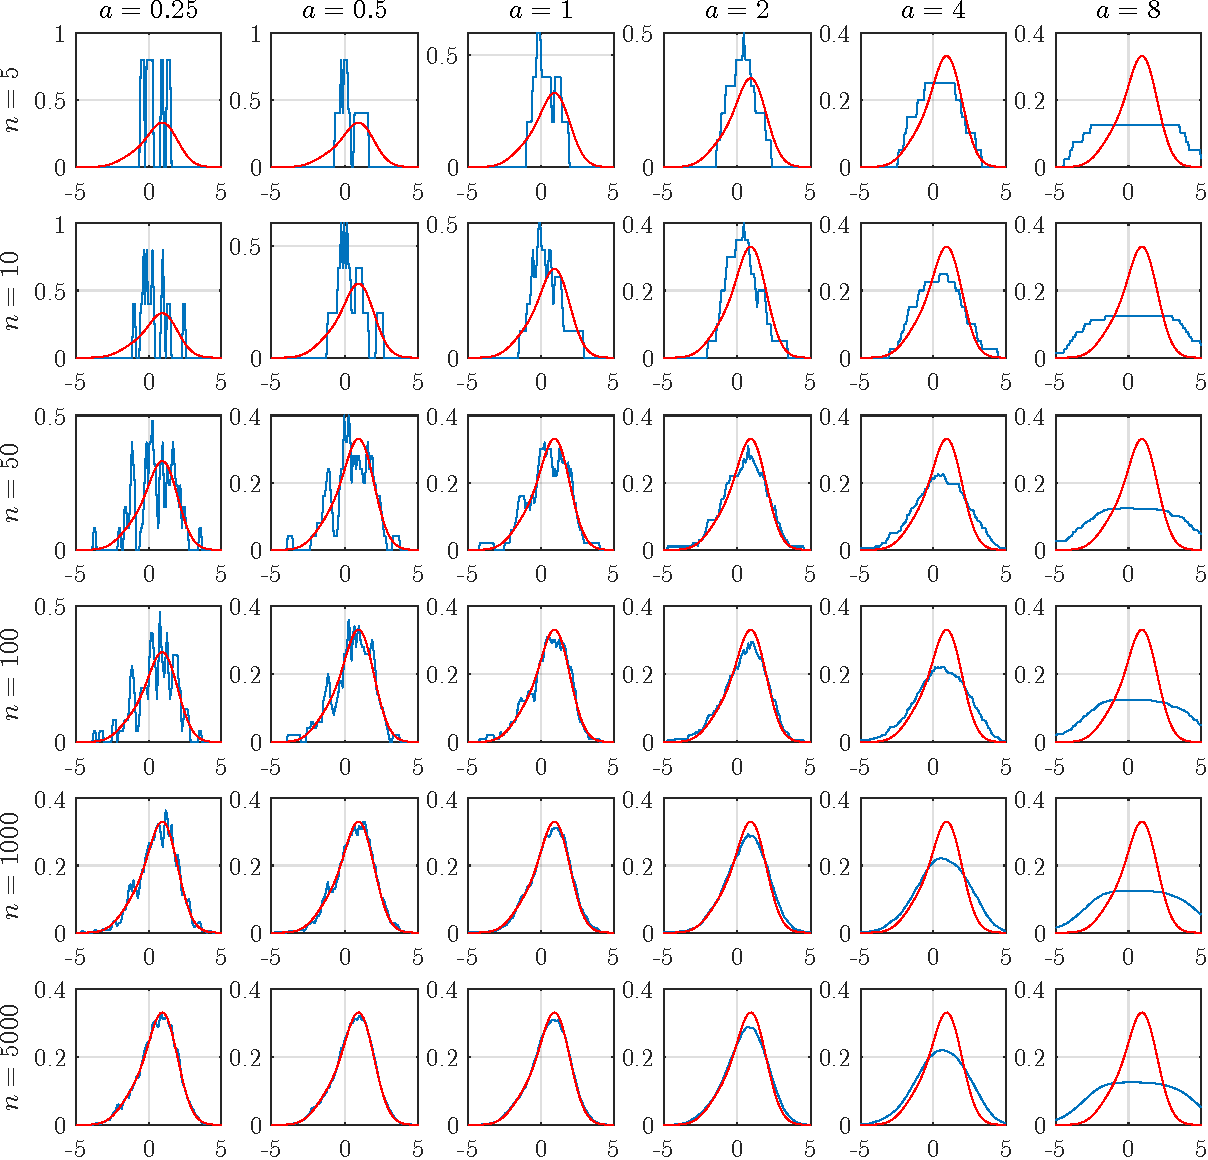
\includegraphics[width=7in]{squareWindow.pdf}
  \caption{方窗估计}
  \label{fig:sqwin}
\end{figure}

(b) Derive how to compute
\begin{equation}
  \epsilon(p_n)=\int\big[p_n(x)-p(x)\big]^2\mathrm{d}x
\end{equation}
numerically.

解: 取积分区间为 [-5, 5], 将区间 $N$ 等分, 记区间长度为 $\Delta \xi$, $\xi_j$ 为第 $j$ 个区间内一点, 当 $N$ 足够大时, 有
\begin{equation}
  \begin{aligned}
    \epsilon(p_n)
    &=\int\big[p_n(x)-p(x)\big]^2\mathrm{d}x\\
    &\simeq\sum_{j=1}^N\big[p_n(\xi_j)-p(\xi_j)\big]^2\Delta \xi\\
    &=\sum_{j=1}^N\left\{\frac{1}{n}\sum_{i=1}^nK(\xi_j-x_i)-\frac{0.2}{\sqrt{2\pi}}\exp\left[-\frac{(\xi_j+1)^2}{2}\right]-\frac{0.8}{\sqrt{2\pi}}\exp\left[-\frac{(\xi_j-1)^2}{2}\right]\right\}^2\Delta \xi\\
  \end{aligned}
\end{equation}

(c) Demonstrate the expectation and variance of $\epsilon(p_n)$ w.r.t different $n$ and $a$.

解: 为了数值计算 $\epsilon(p_n)$ 的期望和方差, 对每一组给定的 $(n,a)$, 进行多次重复试验, 而后对多次试验得到的 $\epsilon(p_n)$ 数组计算均值和方差, 结果分别如表 \ref{tab:squMeanMSE} 和表 \ref{tab:squVarMSE} 所示.

\begin{table}[htbp]
  \centering
  \begin{tabular}{l|cccccc}
  \hline
           & $a=0.25$ & $a=0.5$ & $a=1$  & $a=2$  & $a=4$  & $a=8$  \\ 
  \hline
  $n=5$    & 0.0754   & 0.0344  & 0.0153 & 0.0051 & 0.0038 & 0.0086 \\
  $n=10$   & 0.0377   & 0.0200  & 0.0088 & 0.0035 & 0.0025 & 0.0084 \\
  $n=50$   & 0.0079   & 0.0038  & 0.0017 & 0.0009 & 0.0025 & 0.0083 \\
  $n=100$  & 0.0040   & 0.0016  & 0.0009 & 0.0004 & 0.0019 & 0.0083 \\
  $n=1000$ & 0.0003   & 0.0001  & 0.0001 & 0.0002 & 0.0020 & 0.0083 \\
  $n=5000$ & 0.0001   & 0.0000  & 0.0000 & 0.0002 & 0.0020 & 0.0083 \\ 
  \hline
  \end{tabular}
  \caption{方窗估计均方误差期望}
  \label{tab:squMeanMSE}
\end{table}

\begin{table}[htbp]
  \centering
  \begin{tabular}{l|cccccc}
  \hline
           & $a=0.25$   & $a=0.5$    & $a=1$      & $a=2$      & $a=4$      & $a=8$      \\ \hline
  $n=5$    & 0          & 5.2849e-05 & 5.0611e-05 & 1.1692e-05 & 4.3810e-06 & 1.6058e-07 \\
  $n=10$   & 8.6365e-05 & 5.2020e-05 & 2.4856e-05 & 1.0281e-05 & 5.3322e-07 & 9.2295e-08 \\
  $n=50$   & 5.5701e-06 & 3.1296e-06 & 9.1607e-07 & 5.1668e-07 & 3.5719e-07 & 2.0359e-08 \\
  $n=100$  & 1.4699e-06 & 4.4399e-07 & 1.3575e-07 & 4.8224e-08 & 7.9064e-08 & 5.5102e-09 \\
  $n=1000$ & 6.1293e-09 & 3.7063e-09 & 2.0755e-09 & 5.9962e-09 & 4.8550e-09 & 6.2758e-10 \\
  $n=5000$ & 0          & 4.8334e-41 & 4.8334e-41 & 6.9602e-39 & 0          & 3.1676e-36 \\ \hline
  \end{tabular}
  \caption{方窗估计均方误差方差}
  \label{tab:squVarMSE}
\end{table}

(d) With $n$ given, how to choose optimal $a$ from above the empirical experiences?

解: 由以上经验, 对于给定的 $n$, 可以通过 $\epsilon(p_n)$ 的均值和方差来选取适当的 $a$ 值. 固定 $n$ 时, 随着 $a$ 的增大, 估计效果先变好后变差, 所以 $a$ 在适当的取值下才能最好地逼近真实概率密度函数, 因此可以将 $\epsilon(p_n)$ 的均值与 $a$ 的函数关系绘制出来, 寻找其最小值所在区间, 并在该区间内选择 $\epsilon(p_n)$ 最小方差对应的 $a$.

(e) Substitute $K(x)$ in (a) with Gaussian window. Repeat (a)-(d).

解: 取 $n=5,10,50,100,1000,5000$, $a=0.25,0.5,1,2,4,8$, 使用高斯核函数
\begin{equation}
  K(x)=\frac{1}{\sqrt{2\pi}\sigma}\exp\left[-\frac{x^2}{2\sigma^2}\right]
\end{equation}
进行估计, 其中取 $\sigma=a/\sqrt{n}$, 结果如图 \ref{fig:gauwin} 所示, 图中红色曲线表示 $p(x)$. 对每一组给定的 $(n,a)$, 进行多次重复试验, 而后对多次试验得到的 $\epsilon(p_n)$ 数组计算均值和方差, 结果分别如表 \ref{tab:gauMeanMSE} 和表 \ref{tab:gauVarMSE} 所示.

\begin{figure}[htbp]
  \centering
  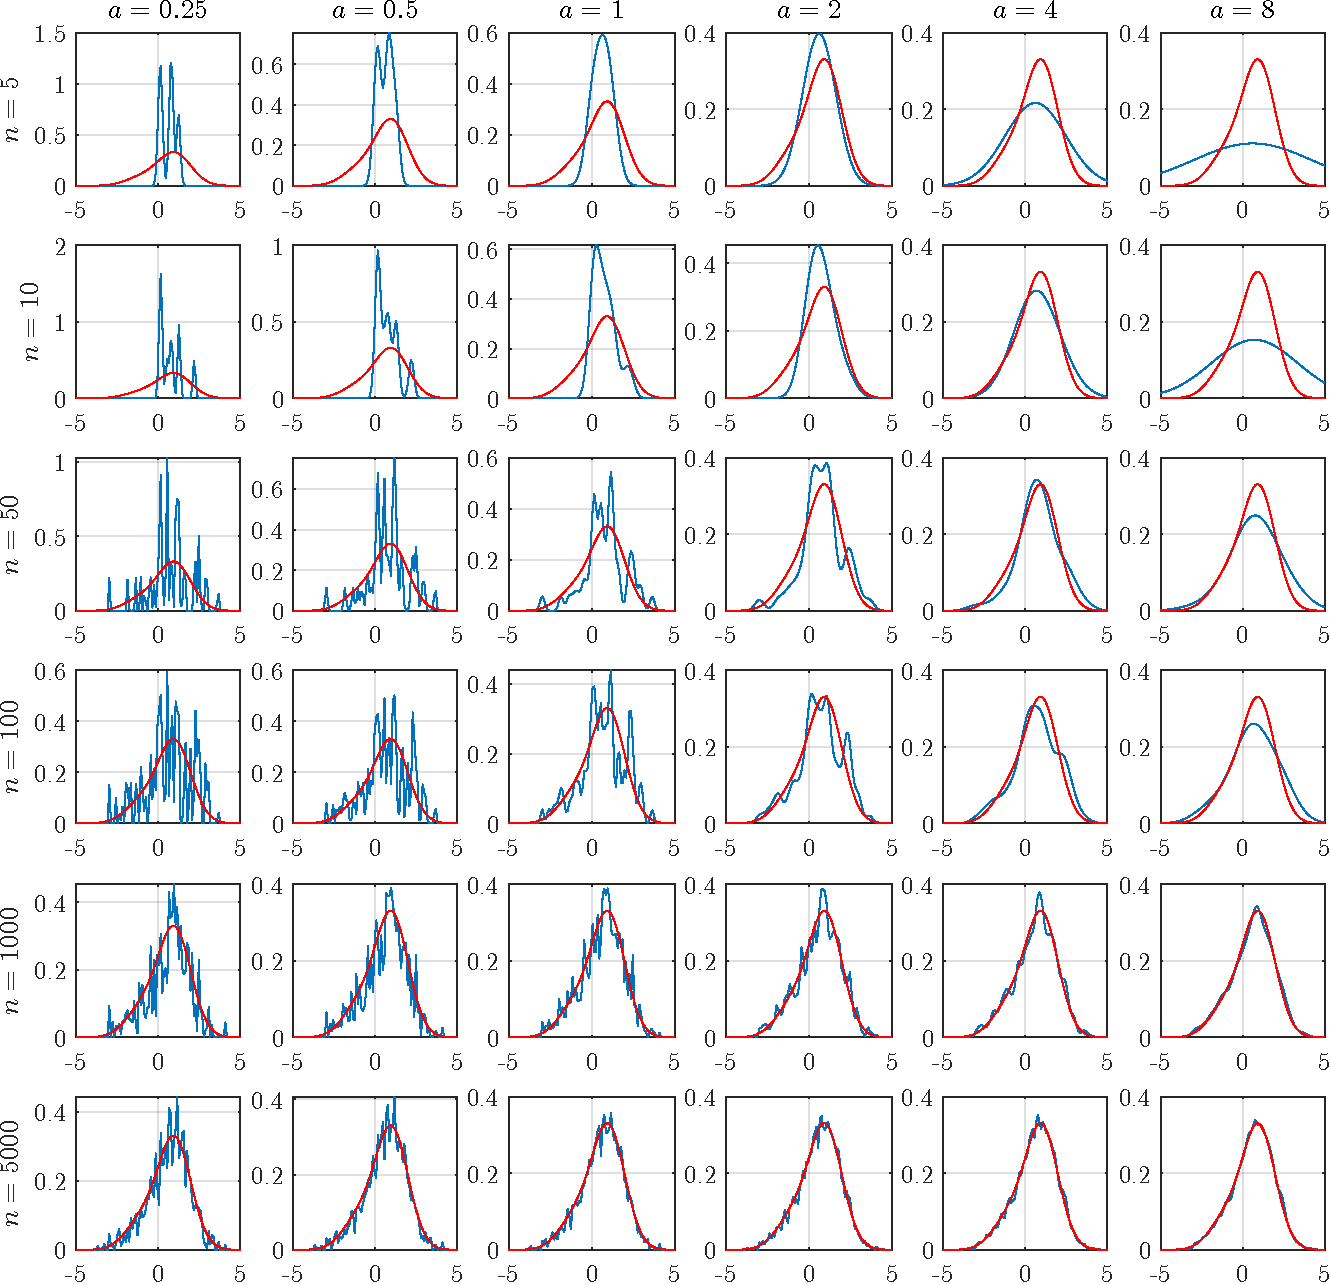
\includegraphics[width=7in]{gaussianWindow.pdf}
  \caption{高斯估计}
  \label{fig:gauwin}
\end{figure}

\begin{table}[htbp]
  \centering
  \begin{tabular}{l|cccccc}
  \hline
           & $a=0.25$ & $a=0.5$ & $a=1$  & $a=2$  & $a=4$  & $a=8$  \\ \hline
  $n=5$    & 0.0440   & 0.0186  & 0.0088 & 0.0055 & 0.0041 & 0.0095 \\
  $n=10$   & 0.0330   & 0.0168  & 0.0062 & 0.0022 & 0.0025 & 0.0065 \\
  $n=50$   & 0.0147   & 0.0077  & 0.0031 & 0.0017 & 0.0007 & 0.0015 \\
  $n=100$  & 0.0110   & 0.0052  & 0.0024 & 0.0011 & 0.0005 & 0.0007 \\
  $n=1000$ & 0.0035   & 0.0019  & 0.0009 & 0.0004 & 0.0002 & 0.0001 \\
  $n=5000$ & 0.0011   & 0.0007  & 0.0003 & 0.0002 & 0.0001 & 0.0000 \\ \hline
  \end{tabular}
  \caption{高斯估计均方误差期望}
  \label{tab:gauMeanMSE}
\end{table}

\begin{table}[htbp]
  \centering
  \begin{tabular}{l|cccccc}
  \hline
           & $a=0.25$   & $a=0.5$    & $a=1$      & $a=2$      & $a=4$      & $a=8$      \\ \hline
  $n=5$    & 8.8794e-05 & 3.5598e-05 & 3.2554e-05 & 5.0078e-05 & 2.1877e-06 & 1.0487e-07 \\
  $n=10$   & 6.2303e-05 & 3.7369e-05 & 6.7287e-06 & 2.0091e-06 & 1.9361e-06 & 1.2545e-07 \\
  $n=50$   & 7.7749e-06 & 9.8888e-06 & 1.4582e-06 & 8.6869e-07 & 1.8728e-07 & 1.7556e-07 \\
  $n=100$  & 9.5059e-06 & 2.0828e-06 & 5.2320e-07 & 3.1134e-07 & 9.8478e-08 & 1.1429e-07 \\
  $n=1000$ & 5.2851e-07 & 9.1313e-08 & 5.3496e-08 & 1.0761e-08 & 5.6957e-09 & 1.6131e-09 \\
  $n=5000$ & 6.6818e-38 & 7.0530e-38 & 1.6240e-38 & 7.4242e-39 & 5.7711e-39 & 5.6068e-39 \\ \hline
  \end{tabular}
  \caption{高斯估计均方误差方差}
  \label{tab:gauVarMSE}
\end{table}

(f) Try different window functions and parameters as many as you can. Which window function/parameter is the best one? Demonstrate it numerically.

解: 取 $n=5,10,50,100,1000,5000$, $a=0.25,0.5,1,2,4,8$, 使用三角形核函数
\begin{equation}
  K(x)=
  \left\{
    \begin{array}{ll}
      \dfrac{1}{a}\left(1-\left\lvert\dfrac{x}{a} \right\rvert\right),&-a\ls x\ls a \\
      0, & \text{otherwise.}
    \end{array}
  \right.
\end{equation}
进行估计, 结果如图 \ref{fig:triwin} 所示, 图中红色曲线表示 $p(x)$. 对每一组给定的 $(n,a)$, 进行多次重复试验, 而后对多次试验得到的 $\epsilon(p_n)$ 数组计算均值和方差, 结果分别如表 \ref{tab:triMeanMSE} 和表 \ref{tab:triVarMSE} 所示.

\begin{figure}[htbp]
  \centering
  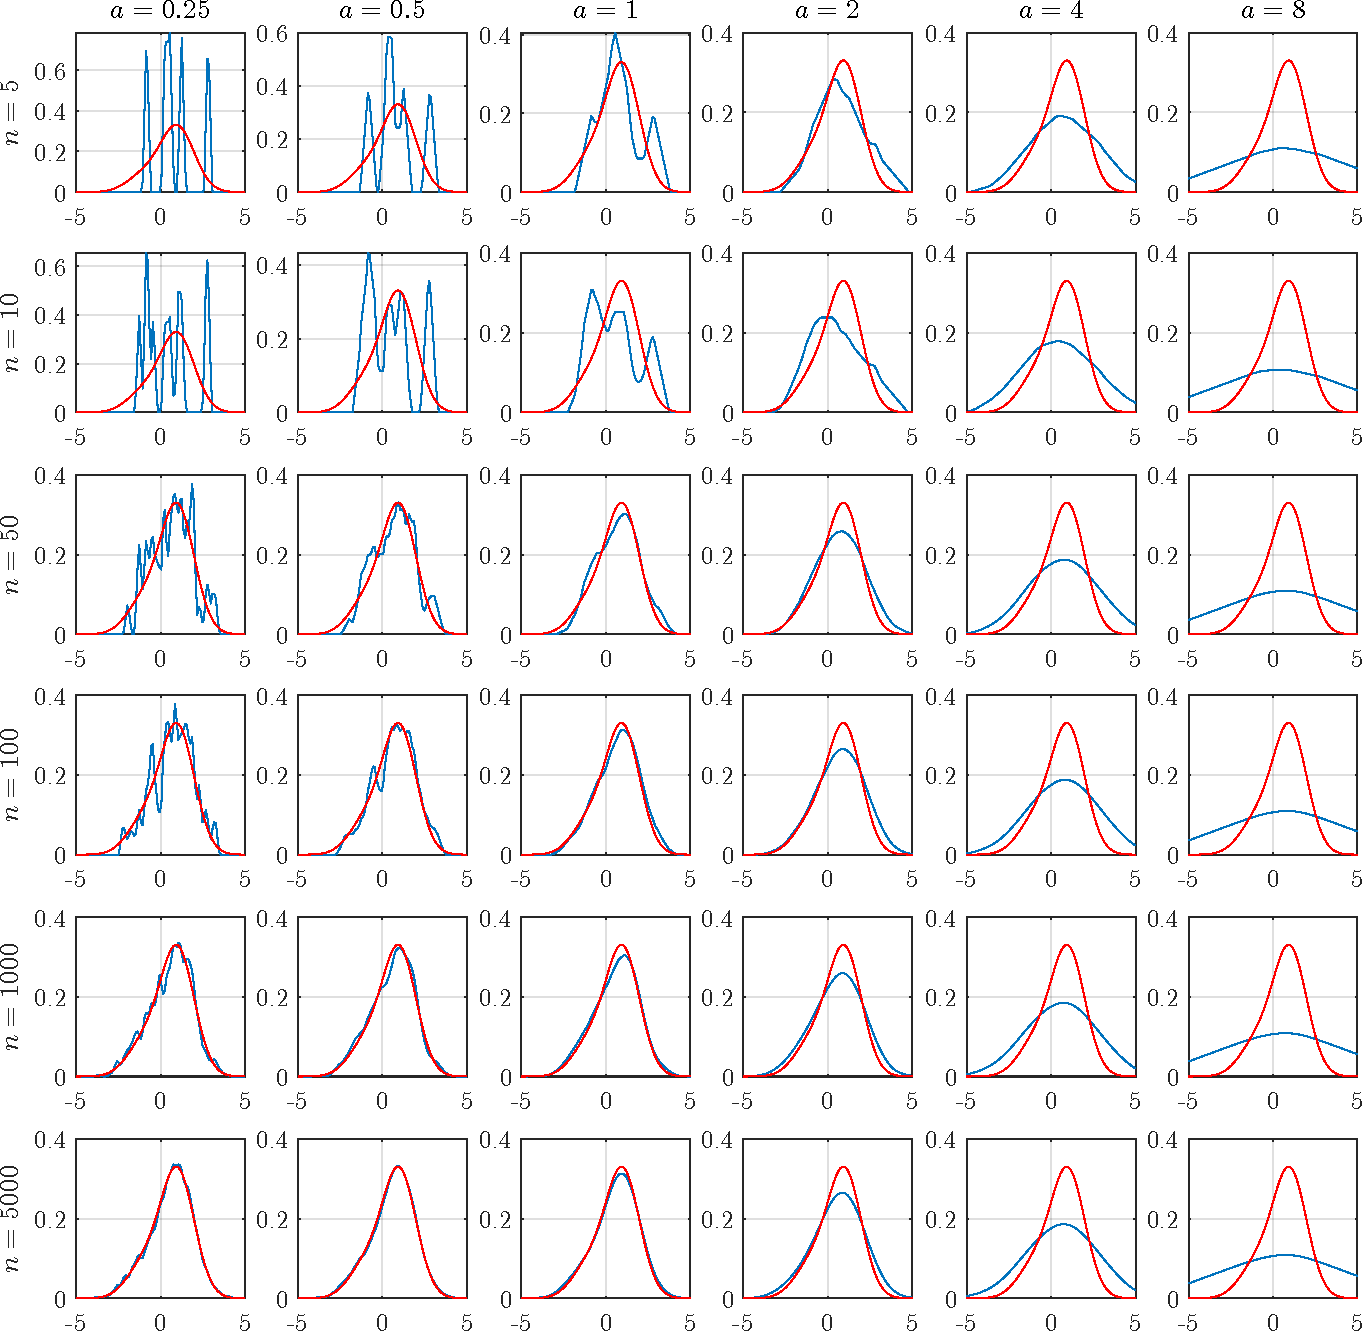
\includegraphics[width=7in]{triangularWindow.pdf}
  \caption{三角形估计}
  \label{fig:triwin}
\end{figure}

\begin{table}[htbp]
  \centering
  \begin{tabular}{l|cccccc}
  \hline
           & $a=0.25$ & $a=0.5$ & $a=1$  & $a=2$  & $a=4$  & $a=8$  \\ \hline
  $n=5$    & 0.0456   & 0.0231  & 0.0085 & 0.0038 & 0.0045 & 0.0092 \\
  $n=10$   & 0.0250   & 0.0113  & 0.0049 & 0.0021 & 0.0038 & 0.0094 \\
  $n=50$   & 0.0050   & 0.0024  & 0.0009 & 0.0011 & 0.0037 & 0.0092 \\
  $n=100$  & 0.0020   & 0.0011  & 0.0005 & 0.0008 & 0.0038 & 0.0092 \\
  $n=1000$ & 0.0002   & 0.0001  & 0.0001 & 0.0006 & 0.0036 & 0.0092 \\
  $n=5000$ & 0.0000   & 0.0000  & 0.0001 & 0.0006 & 0.0036 & 0.0092 \\ \hline
  \end{tabular}
  \caption{三角估计均方误差期望}
  \label{tab:triMeanMSE}
\end{table}

\begin{table}[htbp]
  \centering
  \begin{tabular}{l|cccccc}
  \hline
           & $a=0.25$   & $a=0.5$    & $a=1$      & $a=2$      & $a=4$      & $a=8$      \\ \hline
  $n=5$    & 7.1407e-05 & 1.3686e-04 & 2.7454e-05 & 9.2369e-06 & 1.8634e-06 & 1.6729e-07 \\
  $n=10$   & 4.9860e-05 & 2.2354e-05 & 7.8718e-06 & 4.1982e-06 & 6.1847e-07 & 1.9638e-07 \\
  $n=50$   & 3.1465e-06 & 1.1115e-06 & 2.8525e-07 & 3.0190e-07 & 1.1315e-07 & 1.1064e-08 \\
  $n=100$  & 3.4641e-07 & 1.4459e-07 & 1.6658e-07 & 7.9556e-08 & 7.8658e-08 & 1.0195e-08 \\
  $n=1000$ & 3.8268e-09 & 2.1874e-09 & 1.6549e-09 & 4.0677e-09 & 6.4841e-09 & 8.1923e-10 \\
  $n=5000$ & 1.3256e-39 & 8.1878e-40 & 3.6360e-38 & 1.1693e-37 & 1.0988e-36 & 7.7607e-36 \\ \hline
  \end{tabular}
  \caption{三角估计均方误差方差}
  \label{tab:triVarMSE}
\end{table}

取 $n=5,10,50,100,1000,5000$, $a=0.25,0.5,1,2,4,8$, 使用余弦核函数
\begin{equation}
  K(x)=
  \left\{
    \begin{array}{ll}
      \dfrac{\pi}{4a}\cos\left(\dfrac{\pi x}{2a}\right),&-a\ls x\ls a \\
      0, & \text{otherwise.}
    \end{array}
  \right.
\end{equation} 
进行估计, 结果如图 \ref{fig:coswin} 所示, 图中红色曲线表示 $p(x)$. 对每一组给定的 $(n,a)$, 进行多次重复试验, 而后对多次试验得到的 $\epsilon(p_n)$ 数组计算均值和方差, 结果分别如表 \ref{tab:cosMeanMSE} 和表 \ref{tab:cosVarMSE} 所示.

\begin{figure}[htbp]
  \centering
  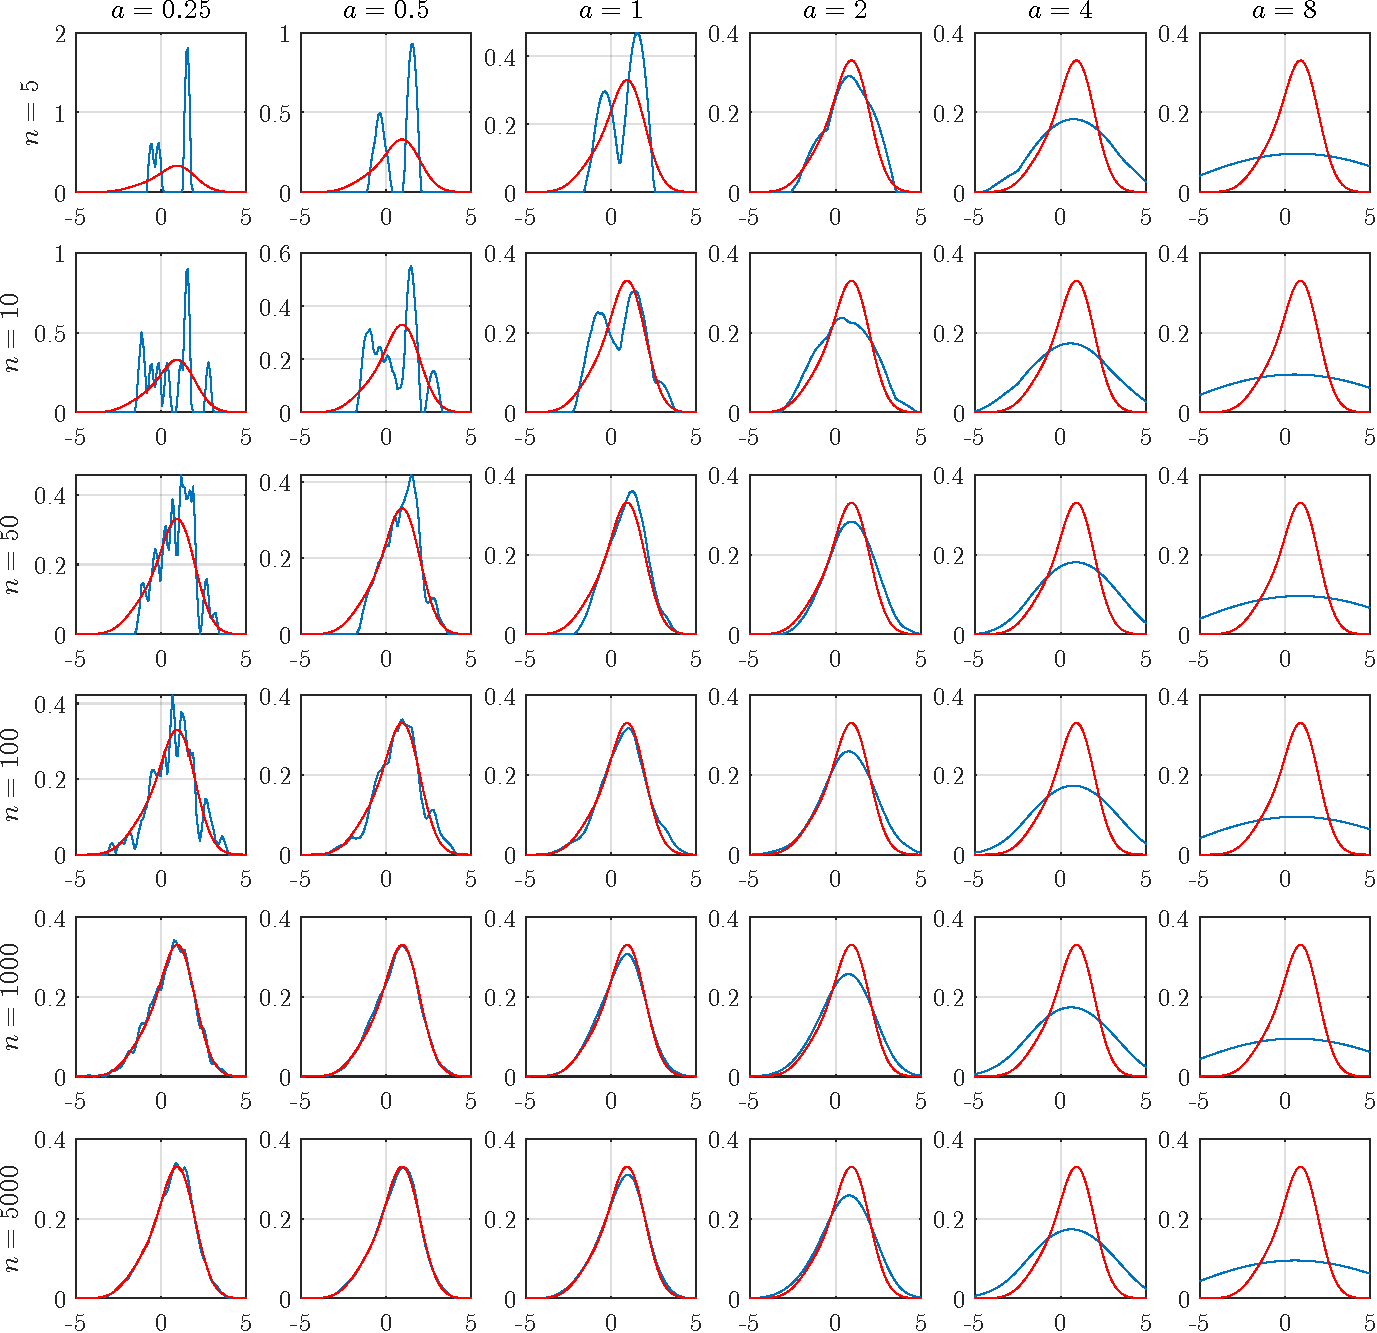
\includegraphics[width=7in]{cosineWindow.pdf}
  \caption{余弦估计}
  \label{fig:coswin}
\end{figure}

\begin{table}[htbp]
  \centering
  \begin{tabular}{l|cccccc}
  \hline
           & $a=0.25$ & $a=0.5$ & $a=1$  & $a=2$  & $a=4$  & $a=8$  \\ \hline
  $n=5$    & 0.0433   & 0.0195  & 0.0068 & 0.0045 & 0.0049 & 0.0106 \\
  $n=10$   & 0.0227   & 0.0104  & 0.0032 & 0.0022 & 0.0044 & 0.0106 \\
  $n=50$   & 0.0047   & 0.0021  & 0.0006 & 0.0009 & 0.0044 & 0.0106 \\
  $n=100$  & 0.0024   & 0.0009  & 0.0005 & 0.0009 & 0.0045 & 0.0106 \\
  $n=1000$ & 0.0002   & 0.0001  & 0.0001 & 0.0008 & 0.0044 & 0.0106 \\
  $n=5000$ & 0.0000   & 0.0000  & 0.0001 & 0.0008 & 0.0044 & 0.0106 \\ \hline
  \end{tabular}
  \caption{余弦估计均方误差期望}
  \label{tab:cosMeanMSE}
\end{table}

\begin{table}[htbp]
  \centering
  \begin{tabular}{l|cccccc}
    \hline
             & $a=0.25$   & $a=0.5$    & $a=1$      & $a=2$      & $a=4$      & $a=8$      \\ \hline
    $n=5$    & 2.2951e-04 & 9.5301e-05 & 1.5815e-05 & 1.9215e-05 & 1.2055e-06 & 4.0842e-08 \\
    $n=10$   & 6.0942e-05 & 2.9110e-05 & 2.7757e-06 & 3.3023e-06 & 2.0050e-07 & 1.4286e-08 \\
    $n=50$   & 3.2806e-06 & 1.3003e-06 & 1.8299e-07 & 2.7372e-07 & 4.0559e-08 & 3.9168e-09 \\
    $n=100$  & 5.7175e-07 & 1.3395e-07 & 1.0991e-07 & 1.0813e-07 & 4.0889e-08 & 1.5858e-09 \\
    $n=1000$ & 3.9053e-09 & 1.2351e-09 & 1.7076e-09 & 5.7179e-09 & 3.2295e-09 & 1.2545e-10 \\
    $n=5000$ & 1.4506e-39 & 1.4286e-39 & 1.4239e-38 & 3.6626e-37 & 1.0295e-36 & 9.5029e-36 \\ \hline
  \end{tabular}
  \caption{余弦估计均方误差方差}
  \label{tab:cosVarMSE}
\end{table}

取 $n=5,10,50,100,1000,5000$, $a=0.25,0.5,1,2,4,8$, 使用指数核函数
\begin{equation}
  K(x)=\frac{1}{2a}\exp\left(-\left\lvert\frac{x}{a}\right\rvert\right)
\end{equation} 
进行估计, 结果如图 \ref{fig:expwin} 所示, 图中红色曲线表示 $p(x)$. 对每一组给定的 $(n,a)$, 进行多次重复试验, 而后对多次试验得到的 $\epsilon(p_n)$ 数组计算均值和方差, 结果分别如表 \ref{tab:expMeanMSE} 和表 \ref{tab:expVarMSE} 所示.

\begin{figure}[htbp]
  \centering
  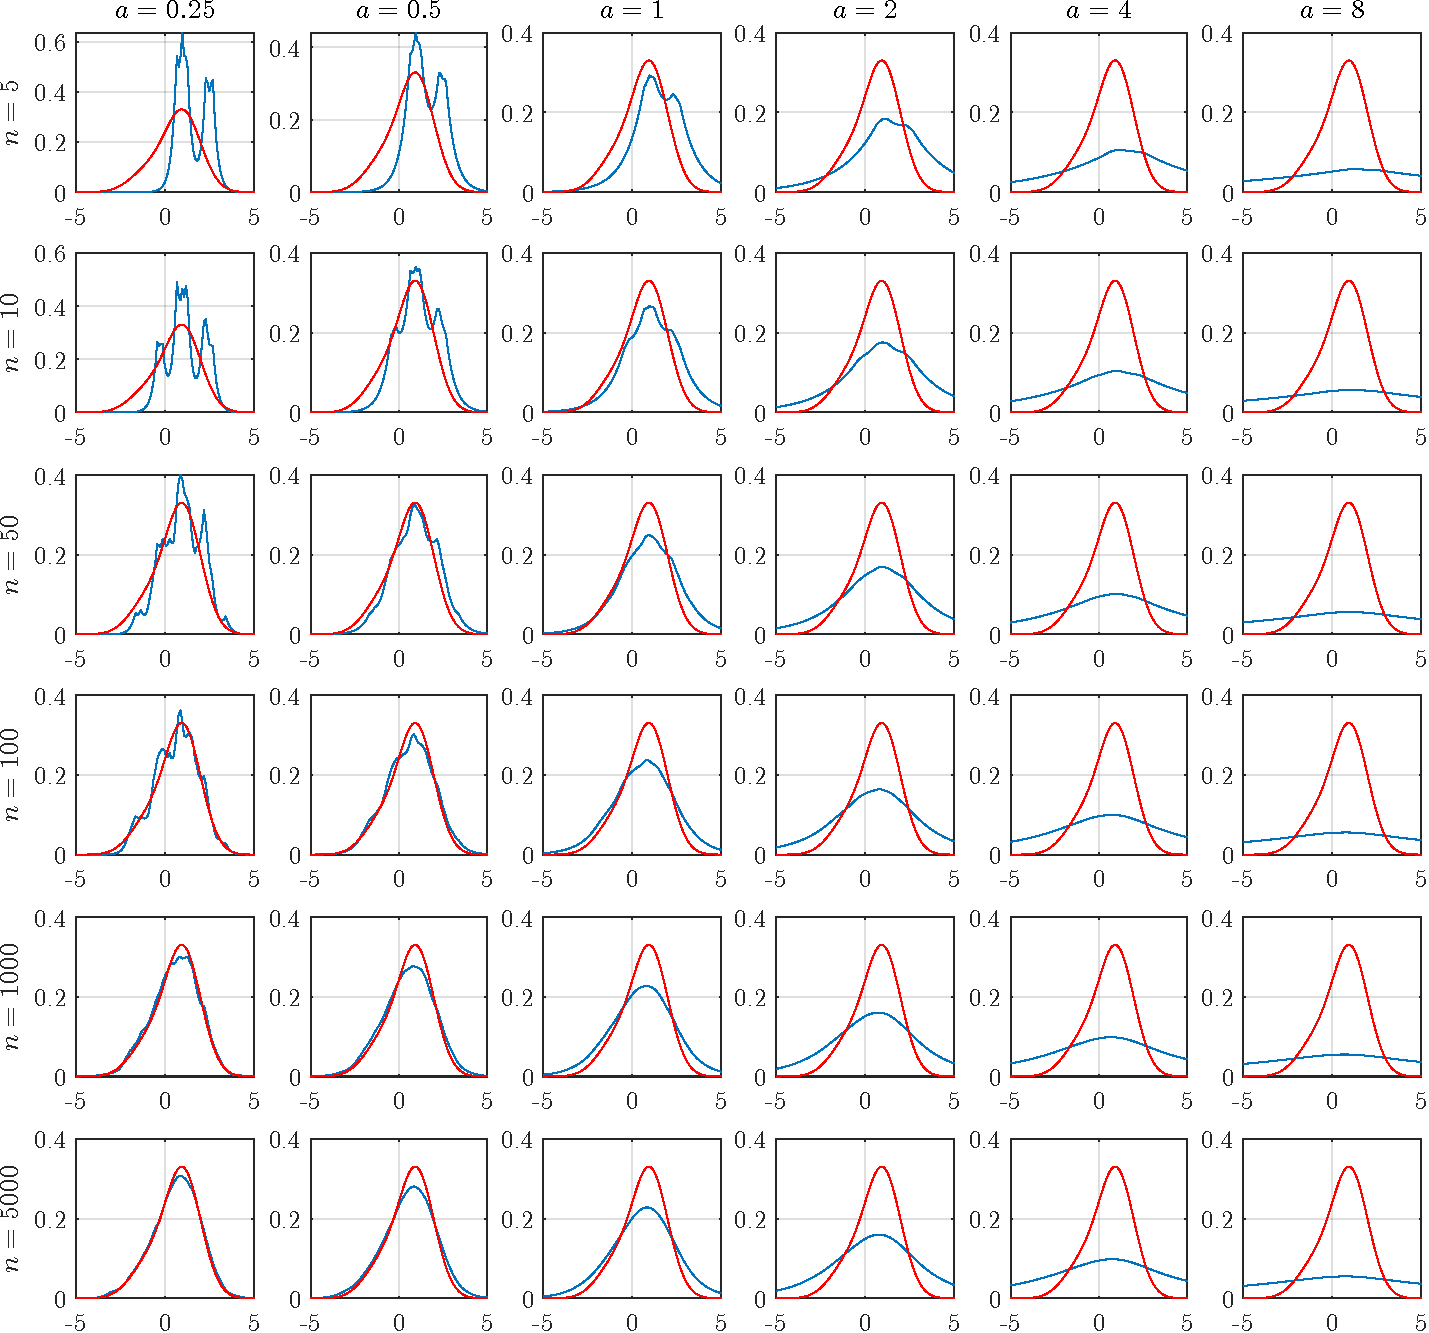
\includegraphics[width=7in]{exponentialWindow.pdf}
  \caption{指数估计}
  \label{fig:expwin}
\end{figure}

\begin{table}[htbp]
  \centering
  \begin{tabular}{l|cccccc}
  \hline
           & $a=0.25$ & $a=0.5$ & $a=1$  & $a=2$  & $a=4$  & $a=8$  \\ \hline
  $n=5$    & 0.0159   & 0.0043  & 0.0029 & 0.0049 & 0.0097 & 0.0139 \\
  $n=10$   & 0.0069   & 0.0034  & 0.0026 & 0.0050 & 0.0097 & 0.0139 \\
  $n=50$   & 0.0015   & 0.0009  & 0.0017 & 0.0049 & 0.0097 & 0.0140 \\
  $n=100$  & 0.0008   & 0.0006  & 0.0016 & 0.0049 & 0.0096 & 0.0140 \\
  $n=1000$ & 0.0001   & 0.0003  & 0.0016 & 0.0050 & 0.0096 & 0.0140 \\
  $n=5000$ & 0.0000   & 0.0003  & 0.0016 & 0.0049 & 0.0096 & 0.0140 \\ \hline
  \end{tabular}
  \caption{指数估计均方误差期望}
  \label{tab:expMeanMSE}
\end{table}

\begin{table}[htbp]
  \centering
  \begin{tabular}{l|cccccc}
  \hline
           & $a=0.25$   & $a=0.5$    & $a=1$      & $a=2$      & $a=4$      & $a=8$      \\ \hline
  $n=5$    & 4.4102e-05 & 4.6225e-06 & 3.6103e-06 & 7.1588e-07 & 6.2318e-07 & 5.3395e-08 \\
  $n=10$   & 4.9972e-06 & 5.7290e-06 & 1.8833e-06 & 8.6840e-07 & 3.0770e-07 & 2.0078e-08 \\
  $n=50$   & 8.6323e-07 & 1.6730e-07 & 3.5128e-07 & 1.9786e-07 & 4.7670e-08 & 5.5717e-09 \\
  $n=100$  & 9.7696e-08 & 1.1821e-07 & 1.8168e-07 & 8.9720e-08 & 1.5764e-08 & 1.6416e-09 \\
  $n=1000$ & 2.5749e-09 & 5.8766e-09 & 1.3514e-08 & 4.2008e-09 & 1.4476e-09 & 2.4628e-10 \\
  $n=5000$ & 7.1807e-39 & 1.7308e-37 & 6.2858e-37 & 4.9494e-36 & 1.1087e-36 & 3.6428e-36 \\ \hline
  \end{tabular}
  \caption{指数估计均方误差方差}
  \label{tab:expVarMSE}
\end{table}

最优参数与窗函数: 通过整体比较方窗, 高斯窗, 三角形窗, 余弦窗, 指数窗等5种类型窗函数的估计效果, 均方误差的期望和方差大小, 可以看出当窗宽 $a=0.5$ 且样本数为 $n=5000$ 时, 三角形窗的估计效果最好, 其均方误差均值 $6.4746\times10^{-6}$ 和方差 $8.1878\times10^{-40}$ 都是所有估计结果中最小的.

% Reference
\begin{thebibliography}{1}
  \bibitem{b1}{Casella, George, and Roger L. Berger. Statistical inference. Cengage Learning, 2021.}
\end{thebibliography}

\end{document}
